\documentclass[a4paper]{article}
%\usepackage[slovene]{babel}
\usepackage[utf8]{inputenc}
\usepackage{amsmath, amssymb, amsfonts}
\usepackage{graphicx}

\begin{document}
\begin{center}
{\LARGE CFD Lab, Worksheet 1} \newline
{\small Zhibin C., Eva B., Wei N.\\}
\end{center}
\begin{enumerate}
\item Observation and visualization of data.\\
After running the simulation with the given input dataset, we obtained the following figure (added are streamlines and velocity vectors) \ref{orig}:

\begin{figure}[h!!]
\centering
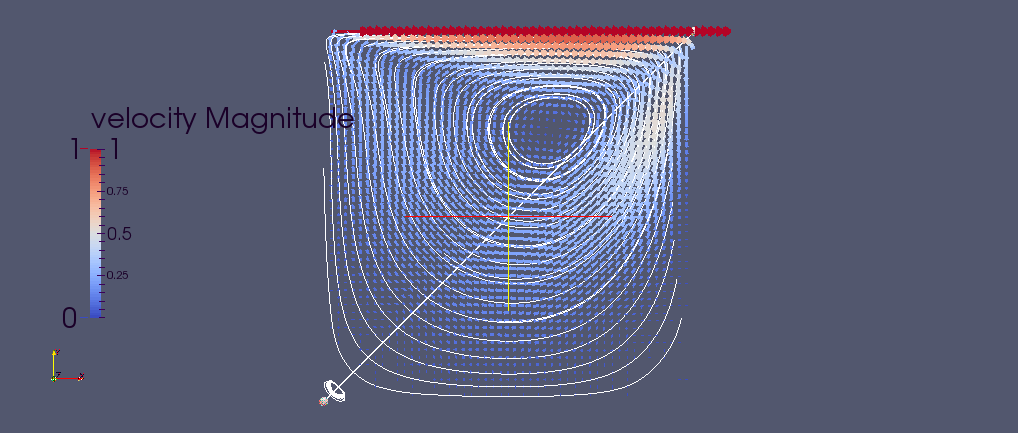
\includegraphics[height= 4cm]{original_simulation.png}
\label{orig}
\caption{Velocity results of the original simulation.}
\end{figure}


\item SOR's behavior depending on $\omega$.\\
We used $omega \in [0, 2]$ using step size $d\omega=0.5$.
Time step size was left unchanged, so that 10000 time steps were made.

\begin{itemize}
\item at $\omega=0$ SOR did not converge(?) (Pressure was left unchanged, the result for velocity is more or less a 
constant state (close to initial); which is a  nonphysical solution. See animation {\textit velocity\_omg0.avi.})
\item at $\omega=0.5$, 1 and $1.5$ we get the expected solution. (should the num. of iterations be checked, to know if it takes longer?)
\item at $\omega=2$ we again lose convergence (in every step of updating pressure matrix we subtract the previous value at the same point...why exactly is
this so bad?). The beginning frames seem correct, but nearing to the end time value we go away from the right end time point solution. See figures \ref{prva}.
\begin{figure}[h!!]
\centering
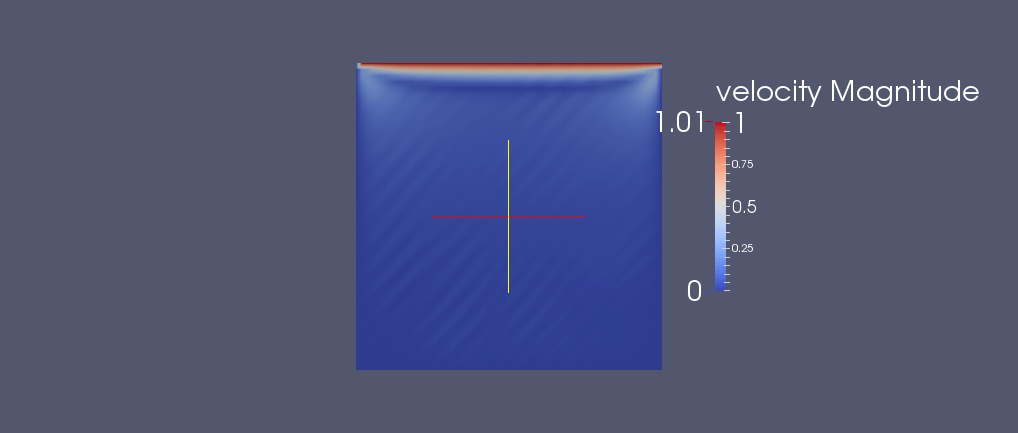
\includegraphics[height= 3.2cm]{velocity_omg2_step0.png}
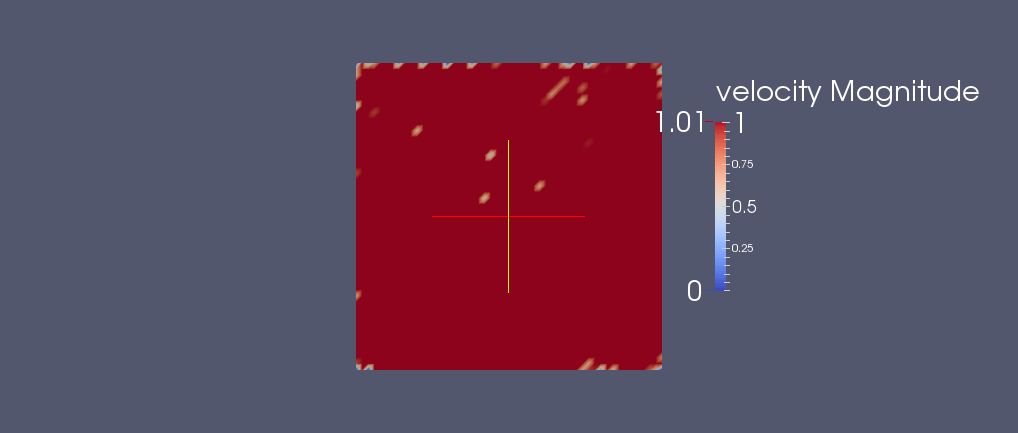
\includegraphics[height= 3.2cm]{velocity_omg2_step1.png}
\label{prva}
\caption{Simulation with $\omega=2$. Left picture is one of the starting frames, and the right one shows trouble in later ones.}
\end{figure}
\end{itemize}

\item Choosing stable time step $dt$.\\
This was done using $\omega=1.7$.
We tried steps from 0.06 to 0.01 (by 0.01), and they were all to big for convergence. When we lowered the step to 0.0095 however, the 
simulation output correct results. After experimenting with 4th and 5th decimal place we saw that the program converged to the right solution with steps 
$\leq 0.00965$, but gives an error at steps $\geq 0.00966$. 

\item Changing space discretization with const. time step.\\ TODO!

\item Effect of viscosity (changing Reynolds number, using adaptive time stepping).\\
After running the program using differen Reynolds' numbers we saw that the liquid behaves quite differently. See figures \ref{reP} of pressures
and \ref{reV} of velocities at the end of our observation, depending on Reynolds number:

\begin{figure}[hbp!]
\centering
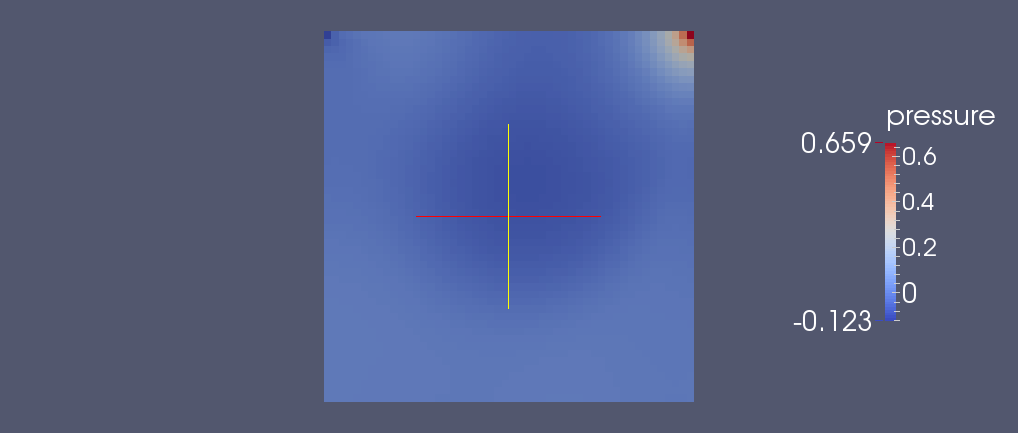
\includegraphics[height= 3.5cm]{Reynolds500_endpressure.png}\\
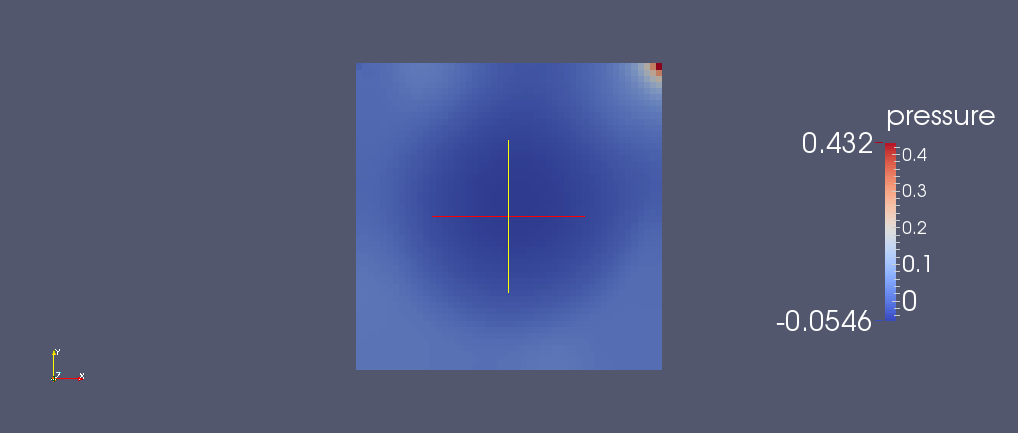
\includegraphics[height= 3.5cm]{Reynolds2000_endpressure.png}\\
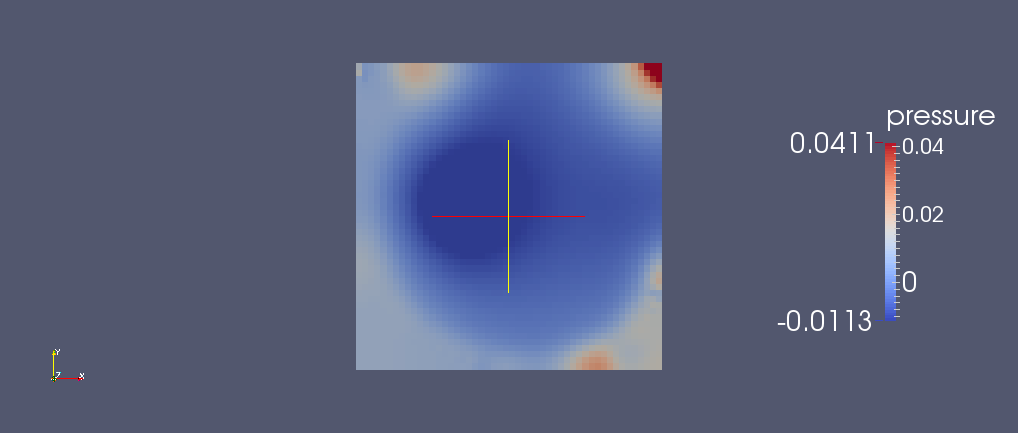
\includegraphics[height= 3.5cm]{Reynolds10000_endpressure.png}
\label{reP}
\caption{State of the pressure at the end, with $Re=500$, $2000$ and $10000$ respectively.}
\end{figure}
\begin{figure}[hbp!]
\centering
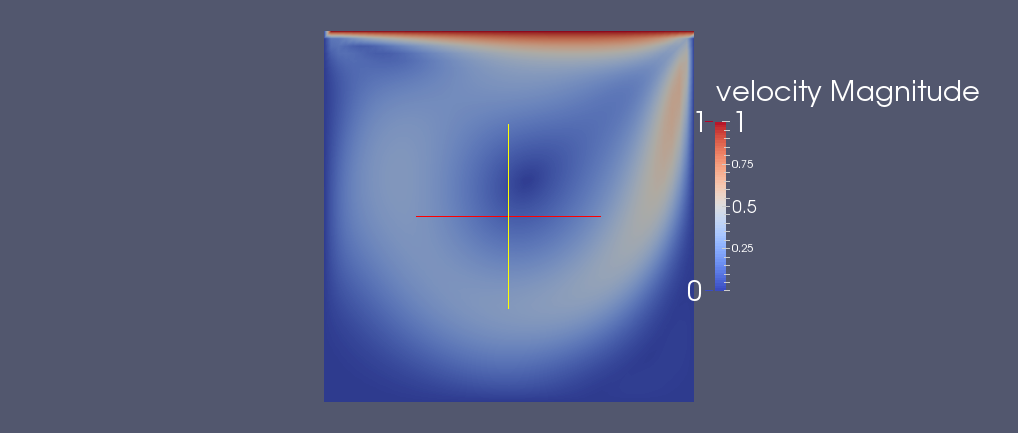
\includegraphics[height= 3.5cm]{Reynolds500_endvelocity.png}\\
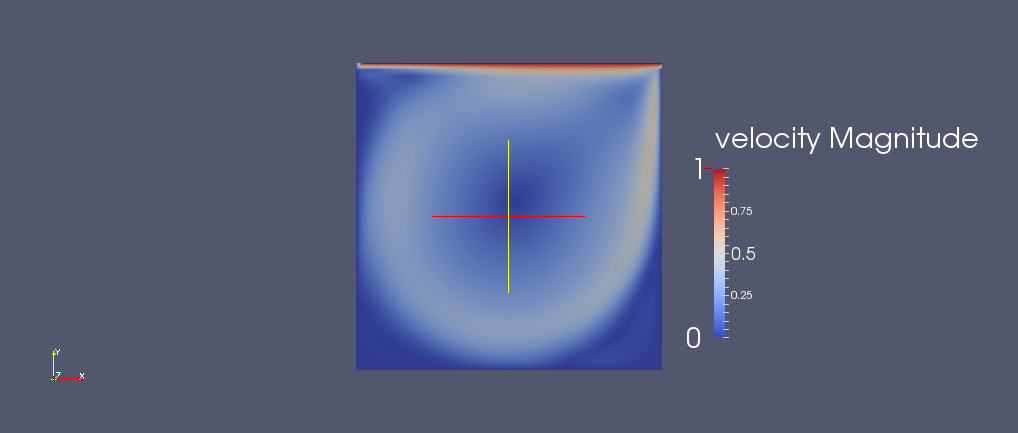
\includegraphics[height= 3.5cm]{Reynolds2000_endvelocity.png}\\
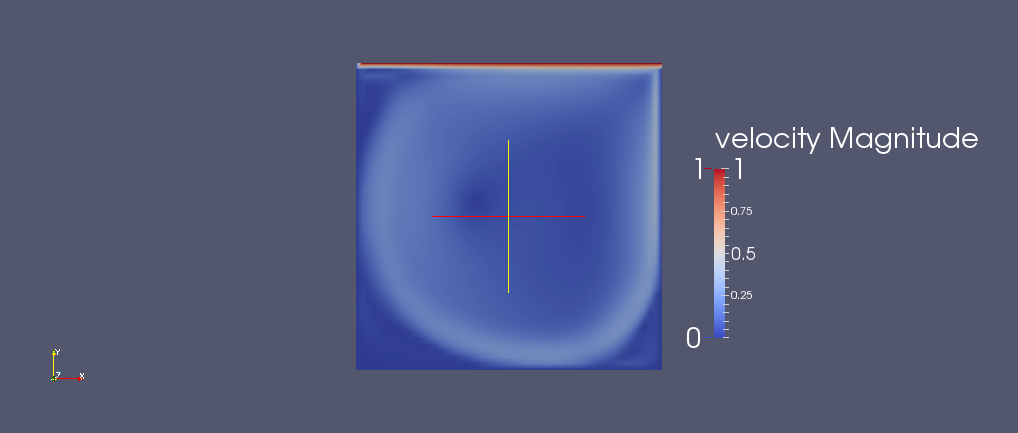
\includegraphics[height= 3.5cm]{Reynolds10000_endvelocity.png}
\label{reV}
\caption{State of the velocity at the end, with $Re=500$, $2000$ and $10000$ respectively.}
\end{figure}



\end{enumerate}

\end{document}
